\documentclass[11pt]{article}
\usepackage{fullpage,amsthm,amsfonts,amssymb,epsfig,amsmath,times,amsthm,enumitem,mathtools,graphicx}

\newtheorem{theorem}{Theorem}
\newtheorem{claim}[theorem]{Claim}
\DeclarePairedDelimiter\ceil{\lceil}{\rceil}
\DeclarePairedDelimiter\floor{\lfloor}{\rfloor}
\graphicspath{{graphs/}}

\begin{document}

\begin{center}
{\bf\Large CMPS 102 --- Winter Quarter 2017 --  Homework 3}\\
{\bf Christopher Hsiao - chhsiao@ucsc.edu - 1398305}
\end{center}

\section*{Solution to Problem 1 - Doing Dishes}

Consider a set $S \text{ of } n$ computer scientist roommates who would like to determine "who will do the dishes after dinner" for the next $m$ nights. Not all roommates have dinner jat home every night, so let $S_i$ denote the subset of roommates who will have dinner at home on the $i^{th}$ night and let $w_i \leq |S_i|$ be the number of people needed to do the dishes on the $i^{th}$ night (some nights multiple people are needed).

For each roommate $j \in S$ and night $1 \leq i \leq m$, let $Q_i(j) = 0$ if $j$ does not eat at home on the $i^{th}$ night, otherwise let $Q_i(j) = w_i/|S_i|$, i.e., if $j$ eats at home on the $i^{th}$ night. Now, for each roommate $j$, let
\begin{equation}
	R_j = \sum_{i=1}^{m} Q_i(j) .
\end{equation}

Clearly, we can't hope that everyone does dishes exactly $R_j$ nights since, in general, $R_j$ won't even be an integer.

Nevertheless, the computer scientists claim:
\begin{center}
	There exists a dish-washing plan under which\\
	each roommate $j \in S$ does the dishes at most $\ceil[\big]{R_j}$ times.
\end{center}

Prove the claim. That is, be a computer scientist.

\textbf{Hint:} Formulate as a flow problem between roommates and nights and use the Integrality Theorem.

\noindent\rule{17cm}{0.4pt}

We build the following flow network. There is a node $p_j \in \{p_1, ..., p_n\}$ for each person $j$, and a node $d_i \in \{d_1, ..., d_m\}$ for each day $i$. There is an edge $(p_j, d_i)$ of capacity $1$ if roommate $p_j$ eats at home on night $d_i$, and is thus eligible to do the dishes. We then connect a super-source $s$ to every person node $p_j \in \{p_1, ..., p_n\}$ with an edge $(s, p_j)$ of capacity $\ceil{R_j}$. This represents the max number of times roommate $p_j$ does the dishes. Then, we connect every day node $d_i \in \{d_1, ..., d_n\}$ to a super-sink $t$ with an edge $(t, d_i)$ with capacity $w_i$, representing the number of people needed to do the dishes on the $i^{th}$ night.

\begin{center}
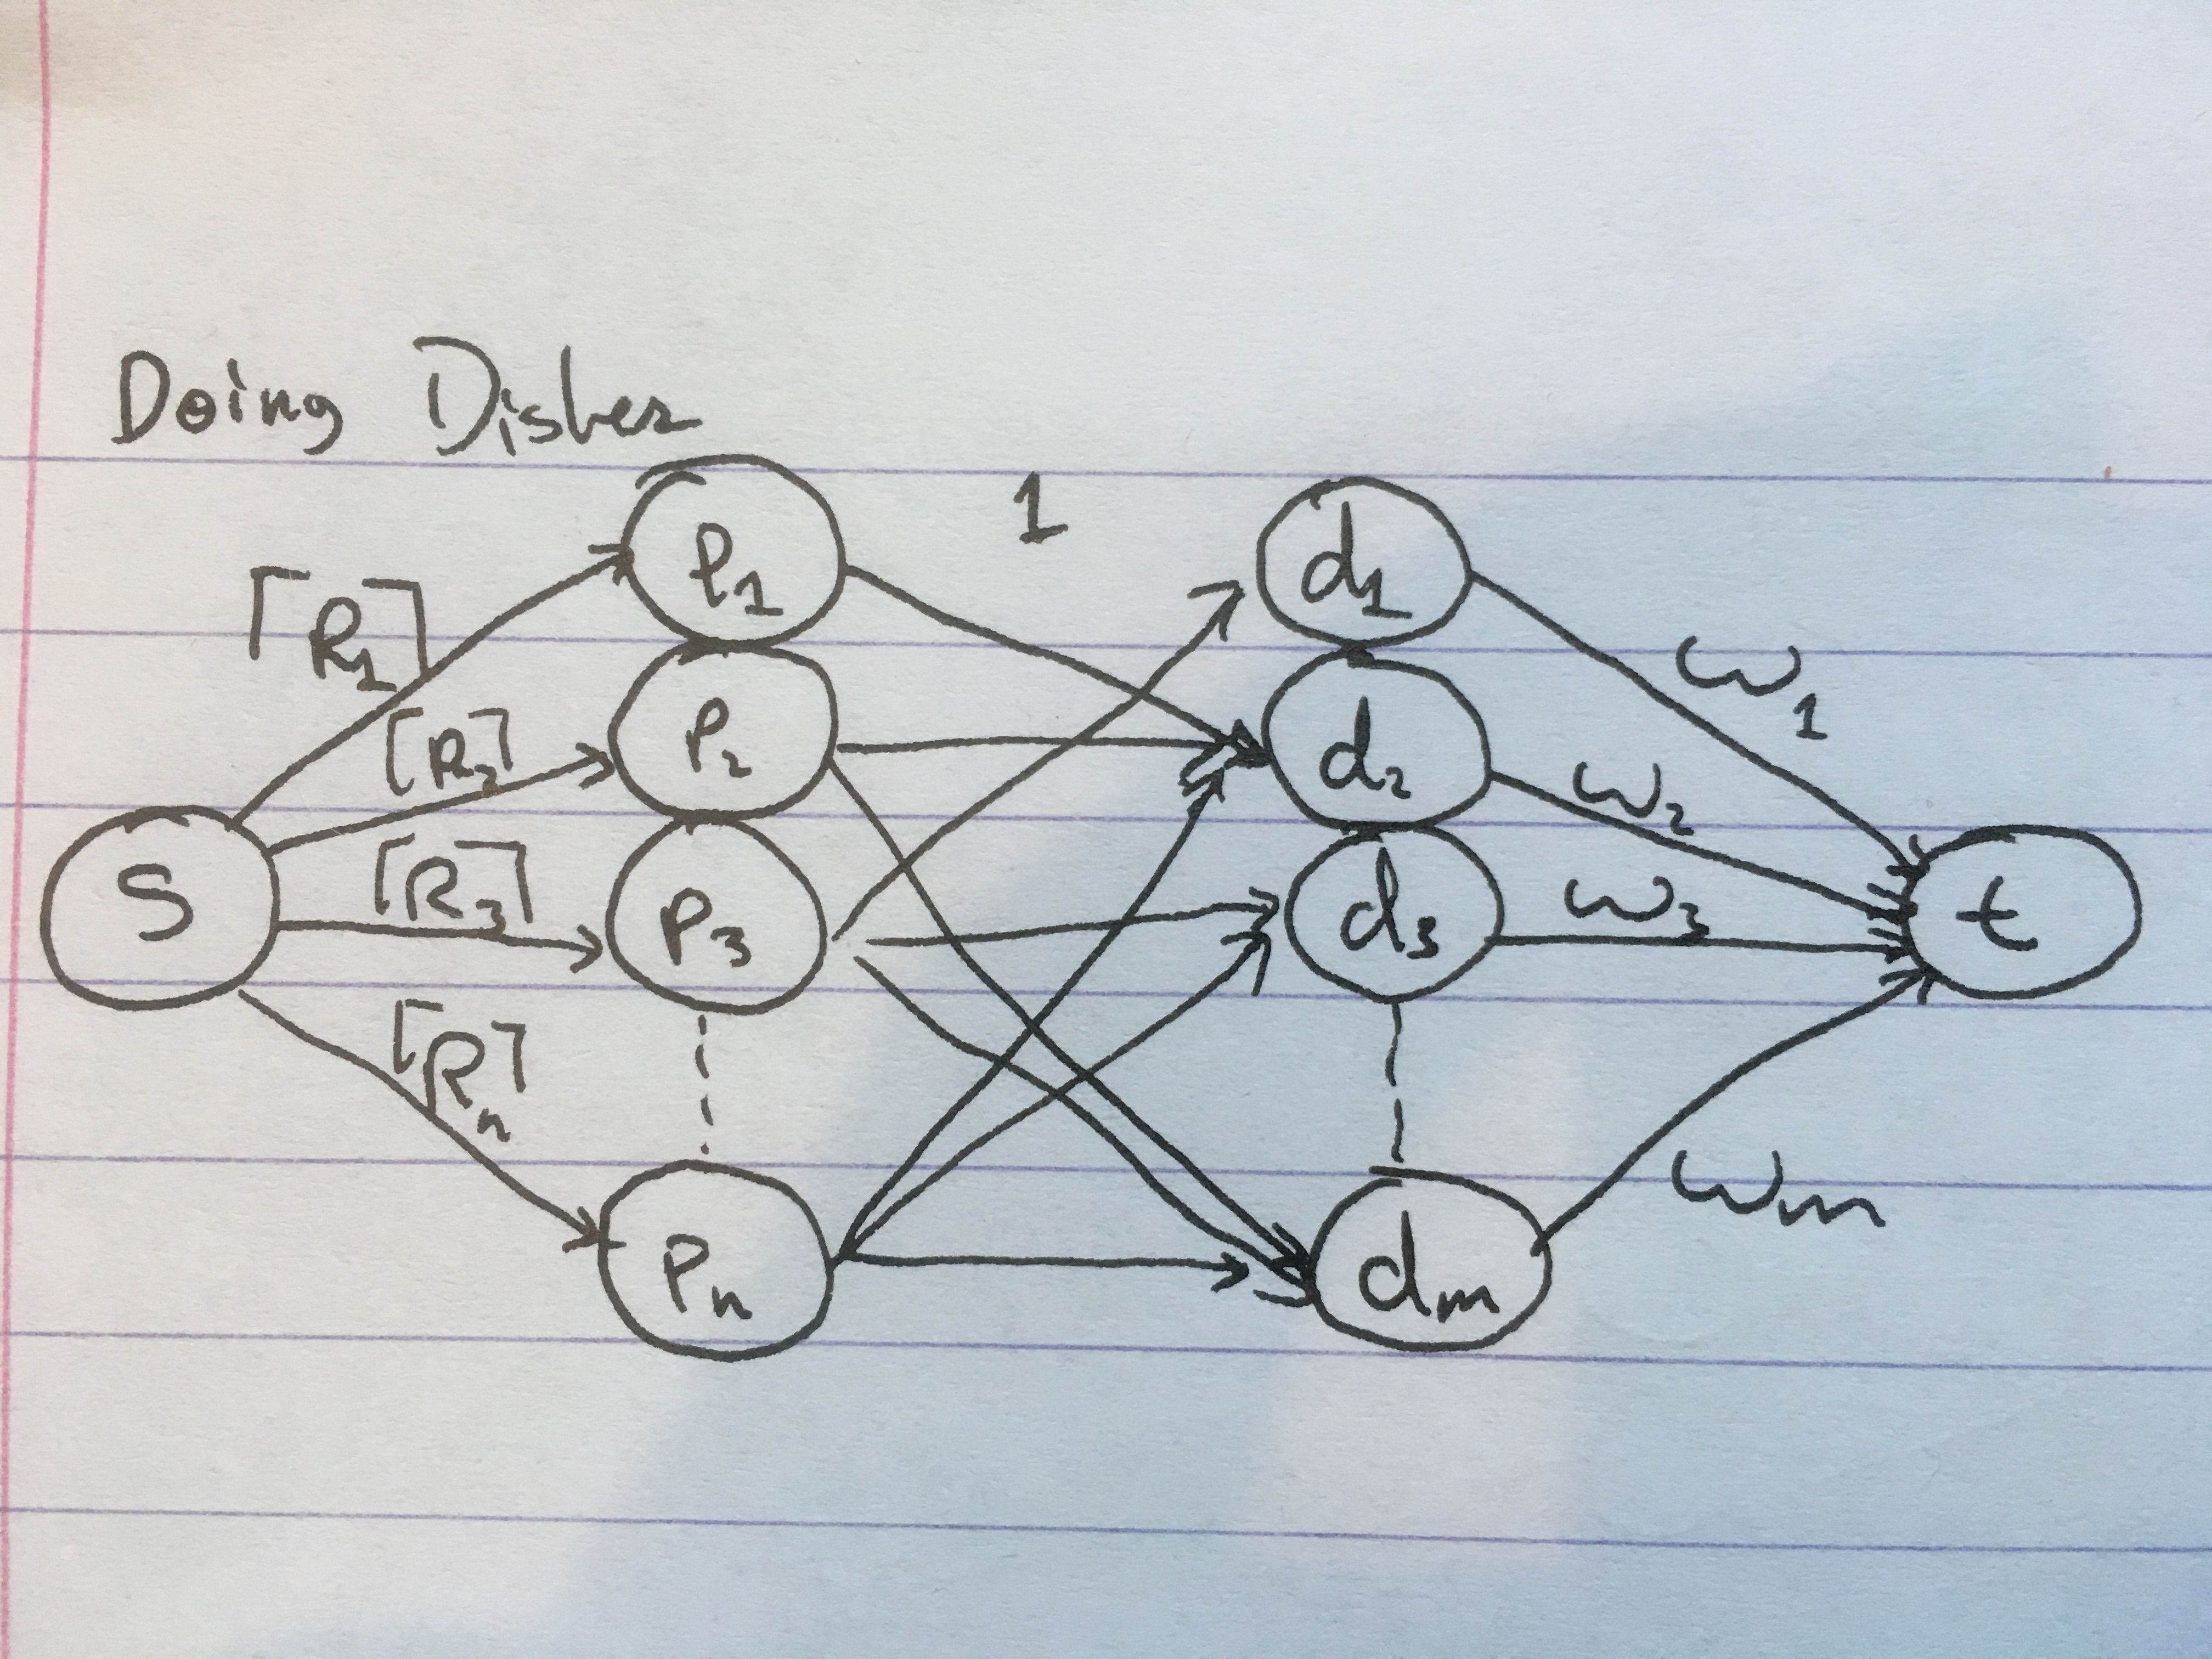
\includegraphics[width=10cm,height=10cm,keepaspectratio]{q1_dishes}
\end{center}

Consider the flow $r = \sum_{j=1}^{n}\ceil{R_j}$. Observe that since $R_j$ is defined as the sum of all $Q_i(j)$, we can rewrite the combined summation as 

\begin{equation}
r = \sum_{j = 1}^{n}\sum_{i=1}^{m}Q_i(j) = \sum_{i=1}^{m} (w_i/|S_i|) \cdot |S_i| = \sum_{i=1}^{m} w_i
\end{equation}

This implies that the sum of all flows across nodes $(s, p_j)$ must equal the sum of all $R_j$'s, which is the sum of all $w_i$'s, which we will call $r$.

\begin{claim}
There exists a valid assignment with no complaints if and only if r = flow.
\end{claim}
\begin{proof}
There cannot be any flow $f > r$, because the total capacity of the cut across the source $s$ leading to the roommate nodes is $r$. Thus, there cannot be any flow greater than $r$ across the graph.

A max flow of $r$ implies edges from $(s, p_j)$ are saturated, as that is the maximum capacity those edges are capable of carrying.
This also means that the flow was capable of reaching the sink $t$ with no overflow, as we proved that $r$ = sum of all $w_i$'s, which is the capacity of all leaving edges $(w_i, t)$. We can find this max flow using $Ford-Fulkerson$. Note that the flow across the inner edges $(p_j, d_i)$ are not integral, but since our capacities are all integers and our flow $f$ is also an integer, by the Integrality Theorem, we can assign integral flow to all edges representing whether or not a roommate $p_j$ who stayed home on day $d_i$ had to do the dishes on that day with integral value $(0, 1)$.
\end{proof}

\begin{claim}
There cannot exist an assignment of roommates to dishes to be done where max flow f < r where there are no complaints.
\end{claim}
\begin{proof}
If max flow $f < r$, then that implies that for some day $d_i$, the dishes that needed to be done $w_i$ was unsatisfied. Since the total capacity from the $(s, p_j)$ edges equals the total capacity from the $(d_i, t)$ edges, the total number of times people need to do dishes $\sum_{j=1}^{n}\ceil{R_j}$ equals the total number of times people are required to do dishes on any given day $\sum_{i=1}^{m}w_i$. Thus, a flow $f < r$ would imply that not all dishes were done, since there was some subset of roommates that were not present on some subset of days to do the required number of dishes.
\end{proof}

The running time is the time required to solve the max-flow problem on a graph with $O(n+m)$ nodes and $O(n \cdot m)$ edges.

\pagebreak



\section*{Solution to Problem 2 - Fussy Eaters}

You are planning a dinner party for $n$ friends who, naturally, have all sorts of dietary restrictions and allergies. Your plan is to cook some appetizer dishes and some main dishes and portion them so that you end up with $n$ appetizer \textit{portions} and $n$ main \textit{portions}. You email everyone, and for each person $i \in \{1, ... , n\}$ you get back their list $A_i$ of OK-to-eat appetizer dishes and their list $M_i$ of OK-to-eat main dishes.

Design an efficient algorithm that takes as input the number of portions of each dish and the lists $A_i, M_i$, designs a max flow instance, has it solved, and uses the (value of the) maximum flow to decide whether or not it is possible to give each friend an appetizer and a main portion that is OK for them to eat.

\noindent\rule{17cm}{0.4pt}
\subsection*{Appetizers}
We build the following flow network. There is a node $p_i \in \{p_1, ..., p_n\}$ for each person $i$, and a node $a_j \in \{a_1, ..., a_n\}$ for each appetizer $j$. There is an edge $(p_i, a_j)$ of capacity $1$ if appetizer $a_j \in A_i$, where $A_i$ represents the appetizers person $i$ is okay with eating. We then connect a super-source $s$ to every person node $p_i \in \{p_1, ..., p_n\}$ with an edge $(s, p_i)$ of capacity 1. Then, we connect every appetizer node $a_j \in \{a_1, ..., a_n\}$ to a super-sink $t$ with an edge $(t, a_j)$ with capacity 1.

\begin{center}
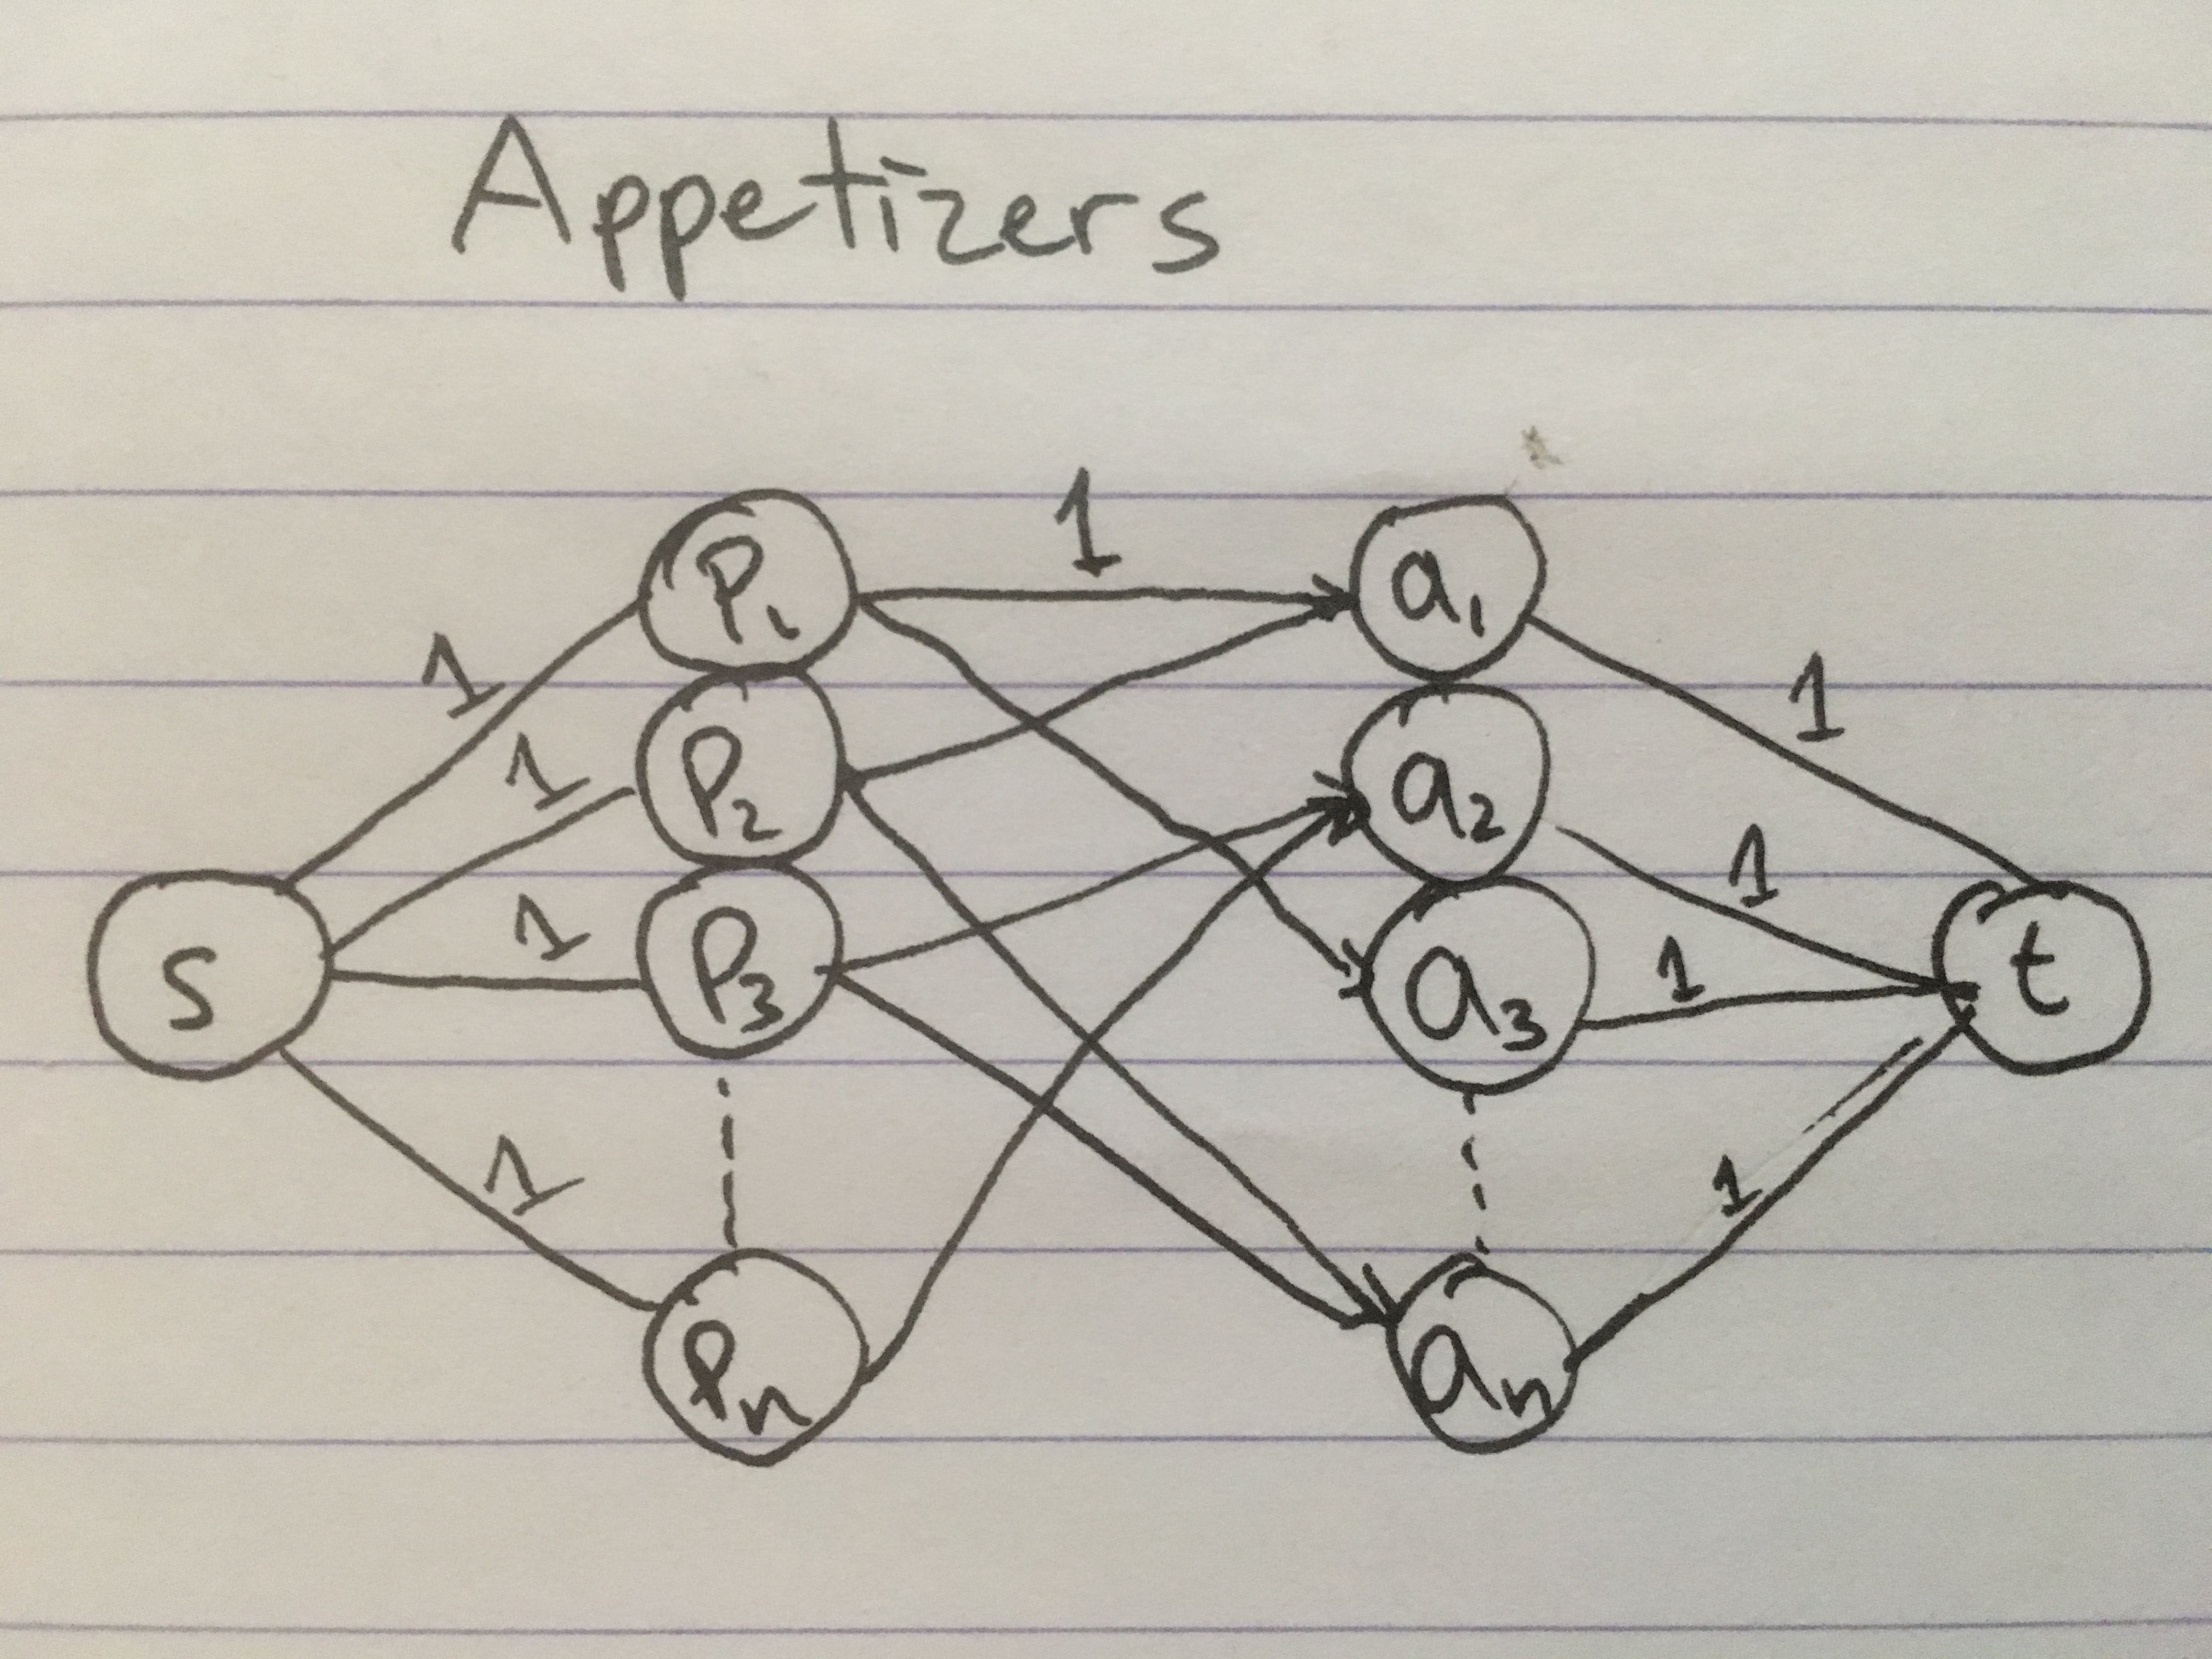
\includegraphics[width=10cm,height=10cm,keepaspectratio]{q2_appetizers}
\end{center}

\begin{claim}
Given a $flow = n$, we can determine an assignment of $n$ people to $n$ dishes such that all people are are satisfied.
\end{claim}

\begin{proof}
There cannot be any $flow > n$, because the total capacity of the cut across the source $s$ leading to the person nodes is $n$. More explicitly, since there are $n$ edges from $s$, each with capacity $1$, there cannot possibly be any flow greater than $n$ across the graph.\\
\\
Now, let us discuss what a max flow of $n$ implies.
\begin{enumerate}
\item All edges $(s, p_i)$ for $i = 1 ... n$ are saturated, as each of the $n$ edges has capacity $1$.
\item All flow was able to traverse the edges $(p_i, a_j)$, such that $n$ flow reaches all $a_j$ nodes.
\item Crucially, there is no "overflow" on any $(a_j, t)$ for $j = 1...n$ edges, as a max flow of $n$ means that all edges directed at $t$ (which have capacity 1) are saturated.
\end{enumerate}

We can find this max flow using $Ford-Fulkerson$. However, note that the flow across the inner edges $(p_i, a_j)$ is distributed, and not necessarily integers. However, by the integrality theorem, since our flow $n$ and all capacities are integral, it then follows that the flow across the inner edges are either $(0, 1)$, with a flow of $1$.
\end{proof}

\begin{claim}
No pairing exists where max flow $< n$ where all guests are satisfied.
\end{claim}
\begin{proof}
From the proof above, we proved that for any flow $f = n$, there exists a stable pairing where no people are dissatisfied. A significant part of the argument was using the saturation of the edges $(a_j, t)$ to represent all appetizers being chosen. For $f < n$, even if the difference $n-f \neq$ some positive integer, it is clear that it is otherwise impossible to saturate some subset of the edges $(a_j, t)$. This means that not all appetizers were able to be "chosen", and some guest was left dissatisfied.. The issue is even more cut and dry when $n-f =$ some integer, because that means only $n-1$ appetizers were chosen, and some guest was left appetizer-less (and dissatisfied). 
\end{proof}

The running time is the time required to solve the max-flow problem on a graph with $O(n+n)$ nodes and $O(n^2)$ edges.


\subsection*{Main Dishes}
\begin{center}
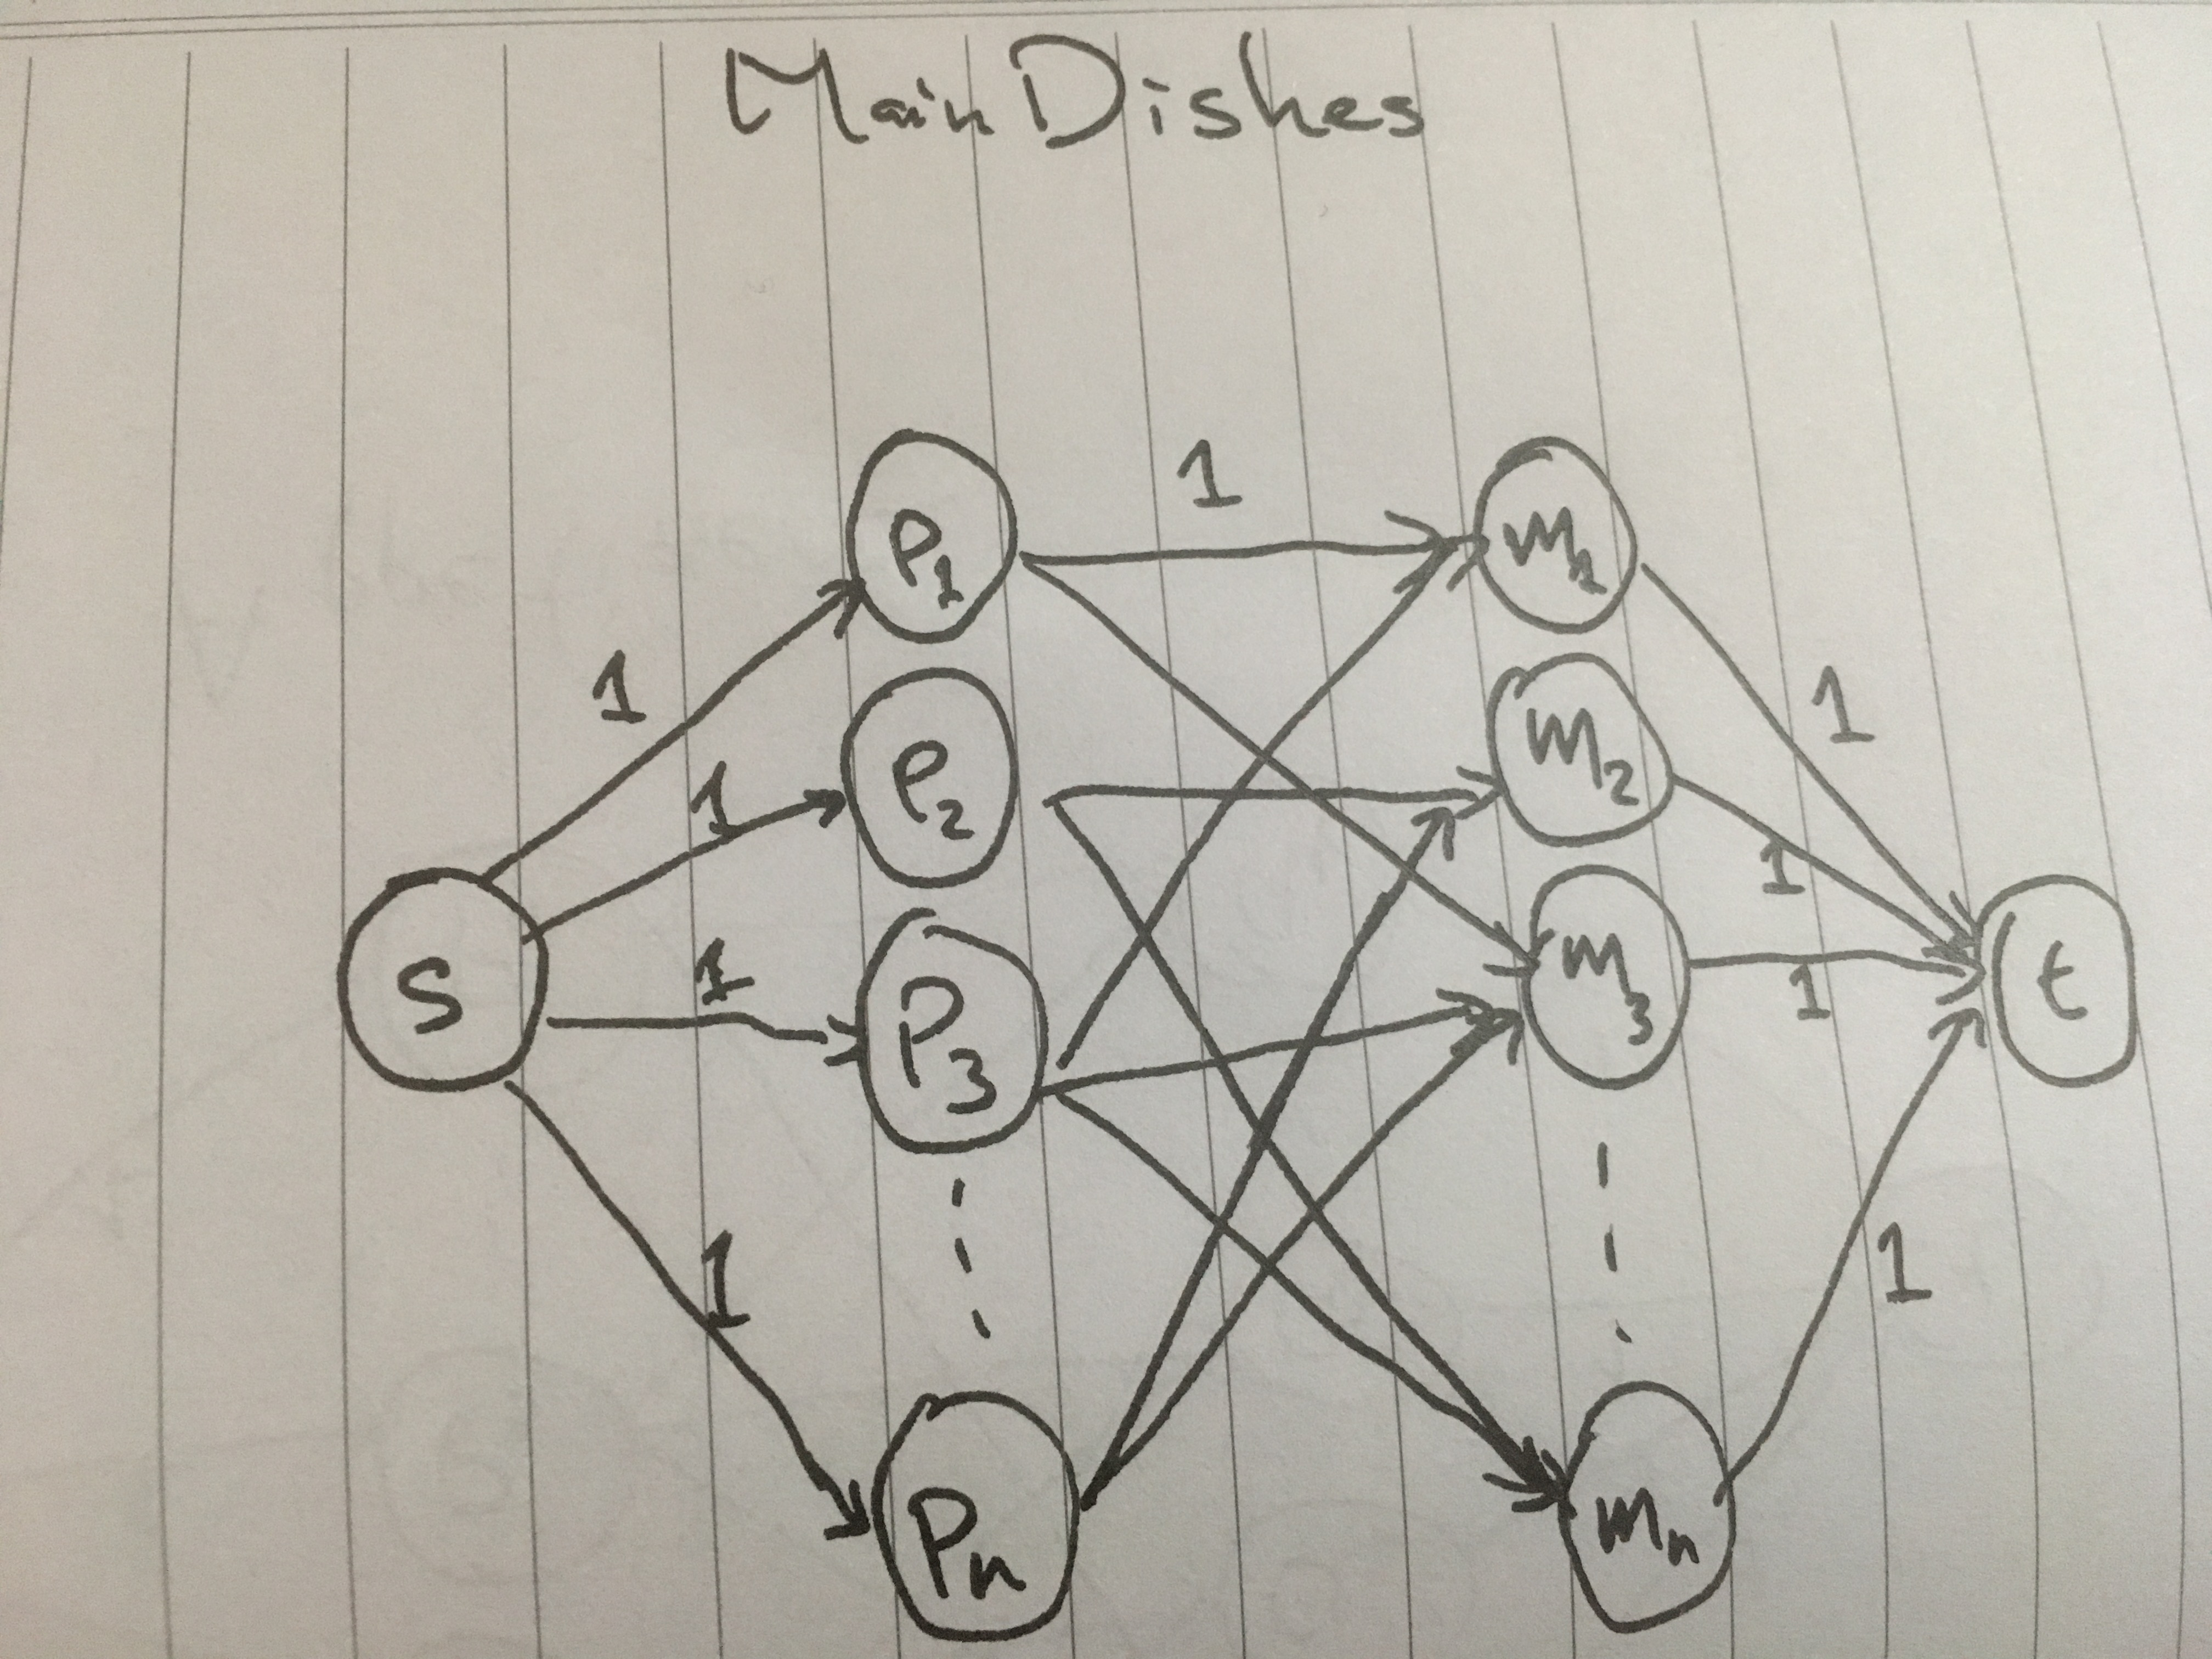
\includegraphics[width=10cm,height=10cm,keepaspectratio]{q2_maindishes}
\end{center}

Observe that for the graph for the Main Dishes, the graph is exactly the same except for the $a_i \in \{a_1,...,a_n\}$ nodes representing appetizers being replaced with the $m_i \in \{m_1, ..., m_n\}$ nodes representing main dishes. Thus, it stands that the graphs are fully analogous, and by extension the proof is also fully analogous.

\pagebreak

\section*{Solution to Problem 3 - Verbal Assault}

You are an English teacher assigning presentations to students. Each of your $n$ students will receive a topic and 31 fancy words that they must use in discussing the topic. You've announced the set of topics $T$ and the set of fancy words $F$, and have received from each student $i \in \{1, ..., n\}$ a set $T_i \subseteq T$ of topics the student is interested in, and a set $F_i \subseteq F$ of fancy words that the student would like to use.

You want to see if it is possible to assign to each student a topic and \textit{exactly} 31 words such that:
\begin{itemize}
	\item Each topic is assigned to at most 2 students.
	\item Each fancy word $w_i$ is assigned to at most $t_i$ students.
\end{itemize}

Describe a method that takes as input the sets $T_i$ and $F_i$ and the number $t_1, ..., t_k$ and returns either "No", or an assignment of topics and words that meets the requirements.

\noindent\rule{17cm}{0.4pt}

\subsection*{Topics}
We build the following flow network to represent the student-topic pairings. There is a node $p_i \in \{p_1, ..., p_n\}$ for each student $i$, and a node $t_j \in \{t_1, ..., t_m\}$ for each topic $j$. There is an edge $(p_i, t_j)$ of capacity $1$ if topic $t_j \in T_i$, where $T_i$ represents the topic student $i$ is okay with writing about. We then connect a super-source $s$ to every student node $p_i \in \{p_1, ..., p_n\}$ with an edge $(s, p_i)$ of capacity 1. Then, we connect every topic node $t_j \in \{t_1, ..., t_m\}$ to a super-sink $t$ with an edge $(t_j, t)$ with capacity 2, representing that each topic can be assigned twice.

\begin{center}
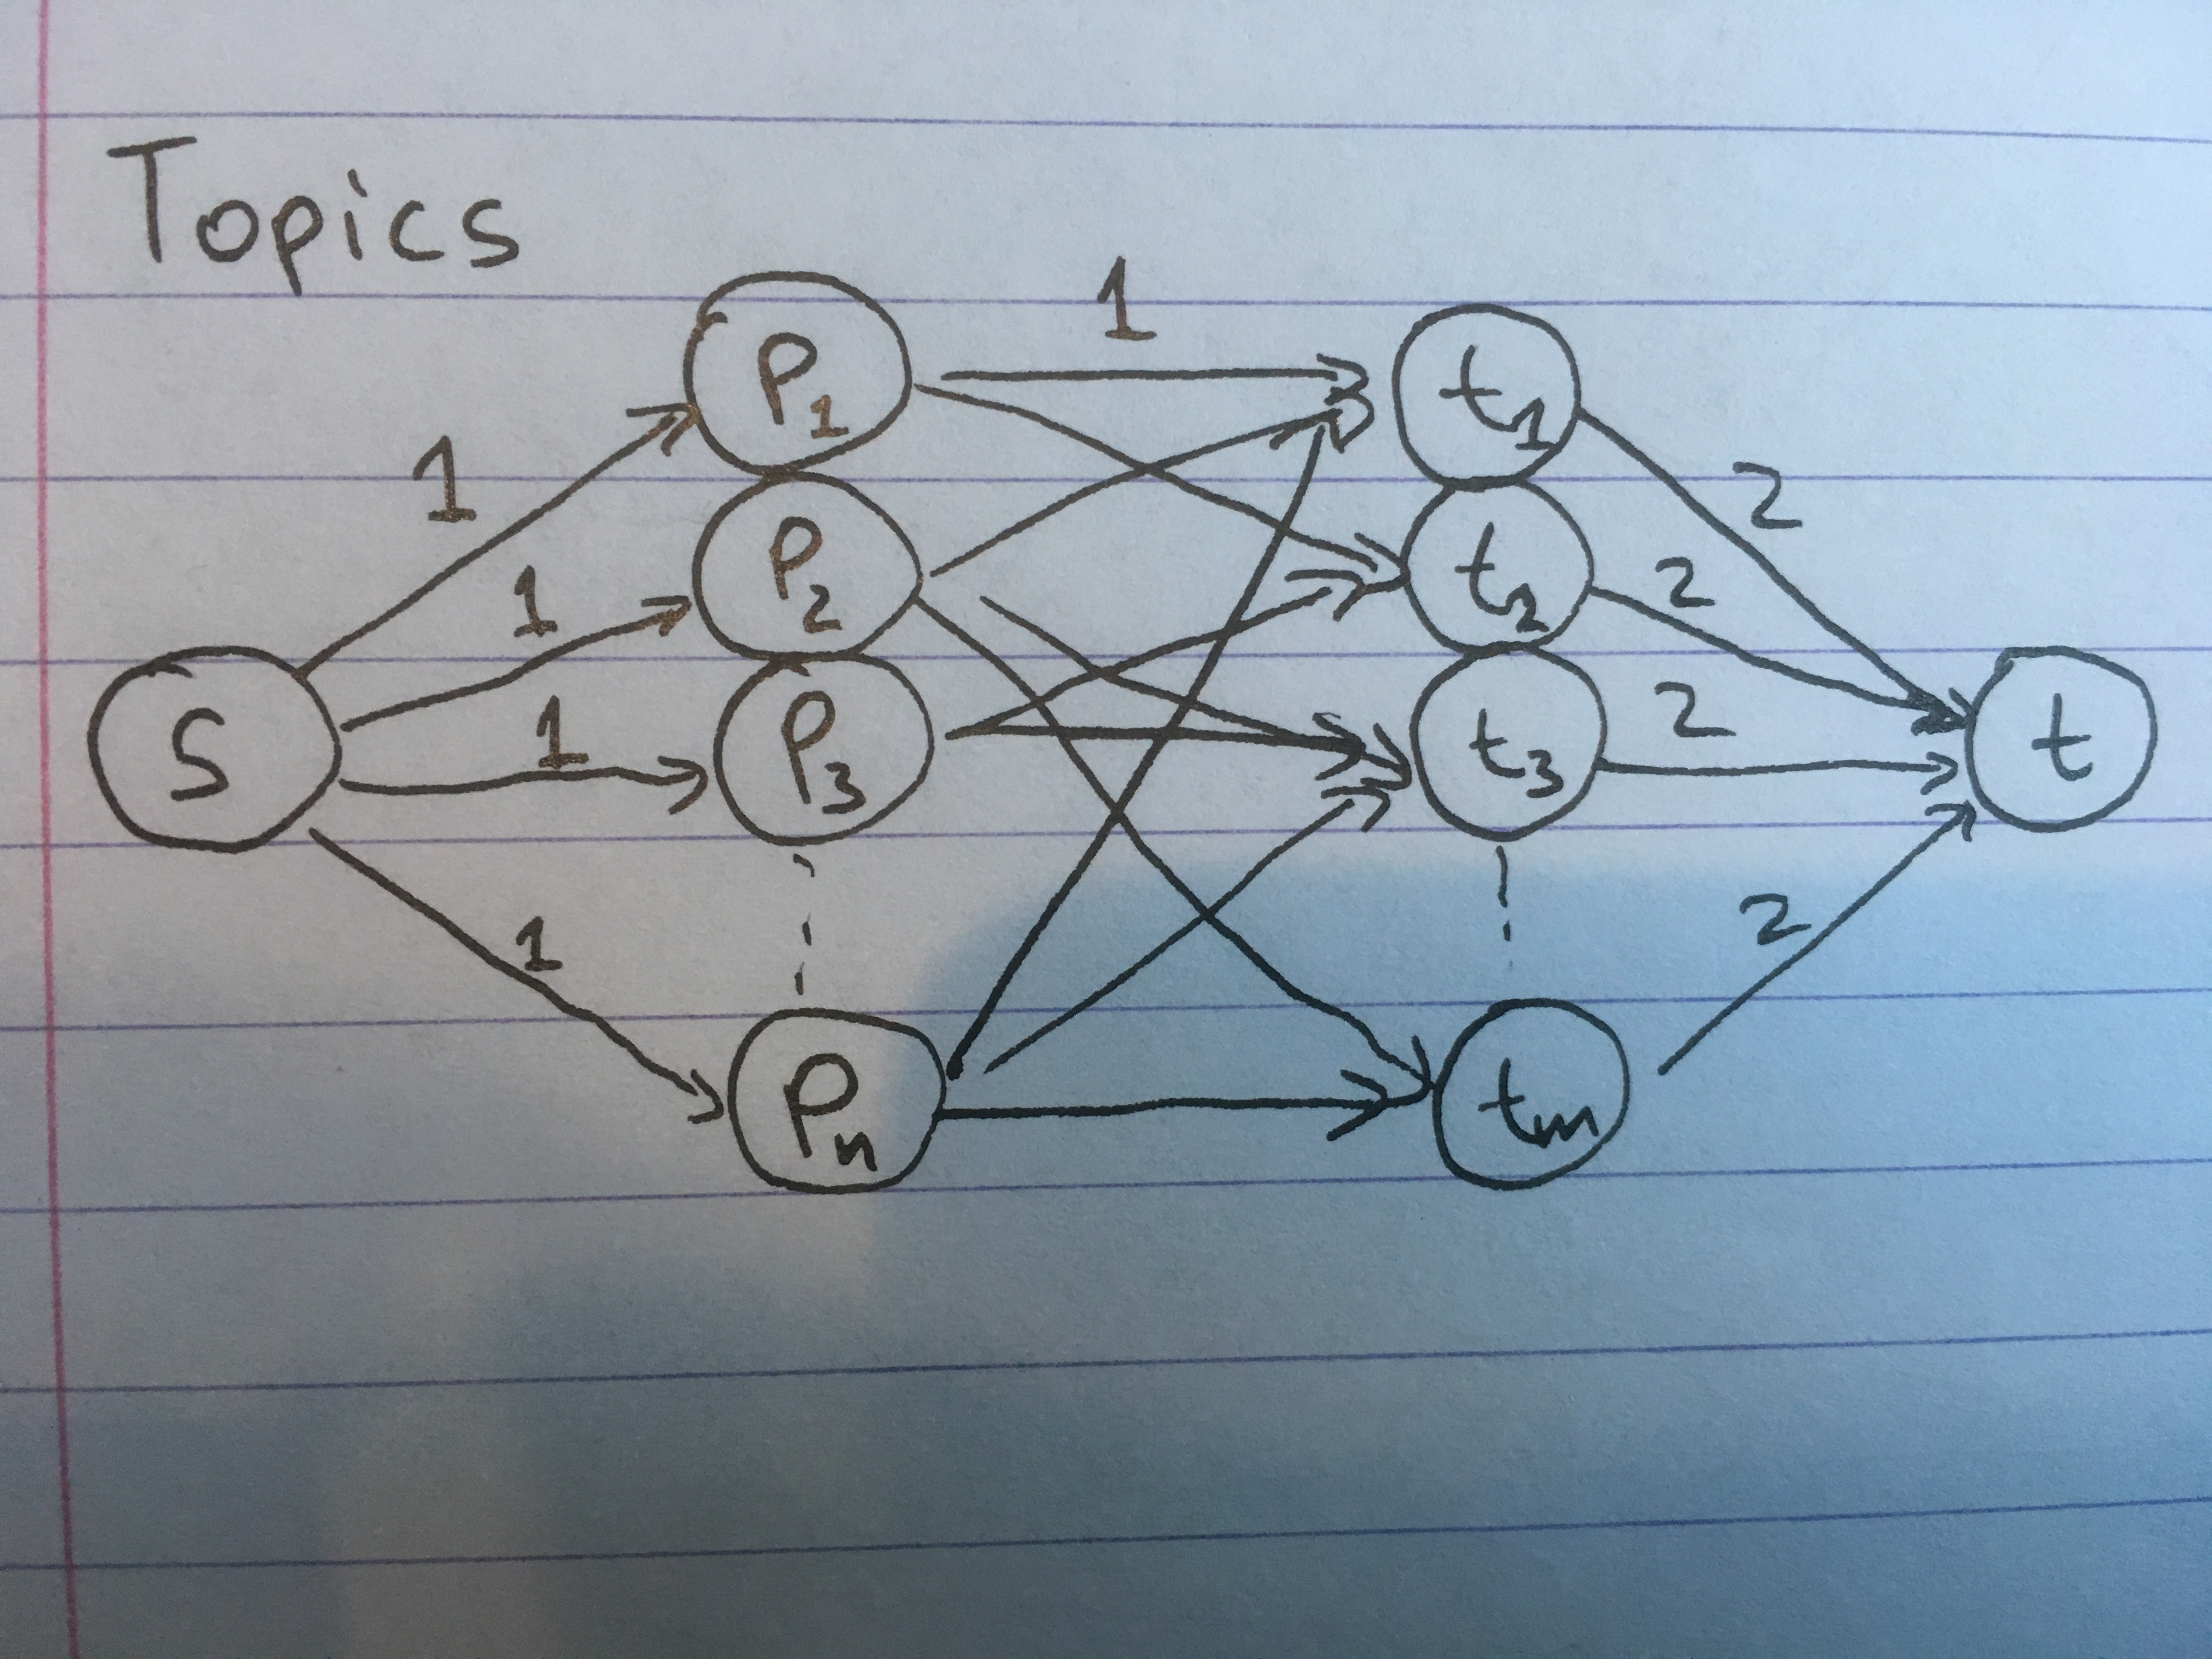
\includegraphics[width=10cm,height=10cm,keepaspectratio]{q3_topics}
\end{center}

\begin{claim}
If and only if we are given a max flow $f = n$ can we construct an assignment of students to topics such that there are no complaints.
\end{claim}
\begin{proof}
$f$ cannot be $> n$, because the flow from $s$ to each student $p_i$ has capacity $1$, and there are $n$ of those edges. Thus, the capacity of the cut on edges $(s, p_i)$ is $n$, and no flow $f > n$ could ever be sent from $s$.

Now, given a max flow $f = n$, we can determine that
\begin{enumerate}
\item All edges $(s, p_i)$ are saturated.
\item All flow was able to flow across all edges $(p_i, t_j)$ for all $i, j$ as well as edges $(t_j, t)$ such that there is no overflow across any edges. There is no overflow across any edge since it means that $n$ flow was able to to traverse the entire system. Note that this does not mean edges $(p_i, t_j)$ or $(t_j, t)$ are saturated.
\end{enumerate}

Knowing this, we can find our max flow $f$ using $Ford-Fulkerson$. Note that flow across inner edges $(p_i, t_j)$ or leaving edges $(t_j, t)$ are not integral. However, since we know that all capacities are integral and our max flow of $n$ is also integral, by the Integrality Theorem, all flow can be assigned an integral value of either $(0, 1)$ across the inner edges, and $(0, 2)$ across leaving edges. Flow of $(0,1)$ across inner edges represents not assigning or assigning a topic to a student respectively, and flow of $(0,2)$ across leaving edges represents the number of times some topic is assigned to a student.
\end{proof}

\begin{claim}
No satisfactory (i.e. 0 complaints) pairing exists for when max flow $f < n$.
\end{claim}
\begin{proof}
If $n-f$ is not an integer, then integrality theorem does not hold, as that means our max flow $f$ is not an integer, then a proper pairing is not possible as student-topic pairings can not be definitively defined. In terms of our problem, a case where $f$ is not an integer cannot properly describe at least one student topic pairing. Thus, some subset of students will be disappointed.

If $n-f$ is an integer, then the case is more straightforward. This means that at least one assignment of student to topic could not be made, even though Integrality Theorem holds. There is at least one student-topic pairing that was not made such that a student could not be paired with a topic, and thus there is guaranteed disappointment. 
\end{proof}

The running time is the time required to solve the max-flow problem on a graph with $O(n+m)$ nodes and $O(nm)$ edges.

\subsection*{Fancy Words}
We build the following flow network to represent the student-fancy word pairings. There is a node $p_i\in \{p_1, ..., p_n\}$ for each student $i$, and a node $w_j \in \{w_1, ..., w_m\}$ for each word $j$. There is an edge $(p_i, w_j)$ of capacity $1$ if word $w_j \in W_i$, where $W_i$ represents the set of fancy words student $i$ has chosen as a word they'd like to use. We then connect a super source $s$ to every student node $p_i \in \{p_1, ..., p_n\}$ , with an edge $(s, p_i)$ of capacity 31, representing the requirement that a student be assigned $31$ words. Then, we connect every word node $w_j \in \{w_1, ..., w_m\}$ to a super-sink $t$ with an edge $(w_j, t)$ with capacity $t_j$, representing the number of times a word can be assigned to a student.
\begin{center}
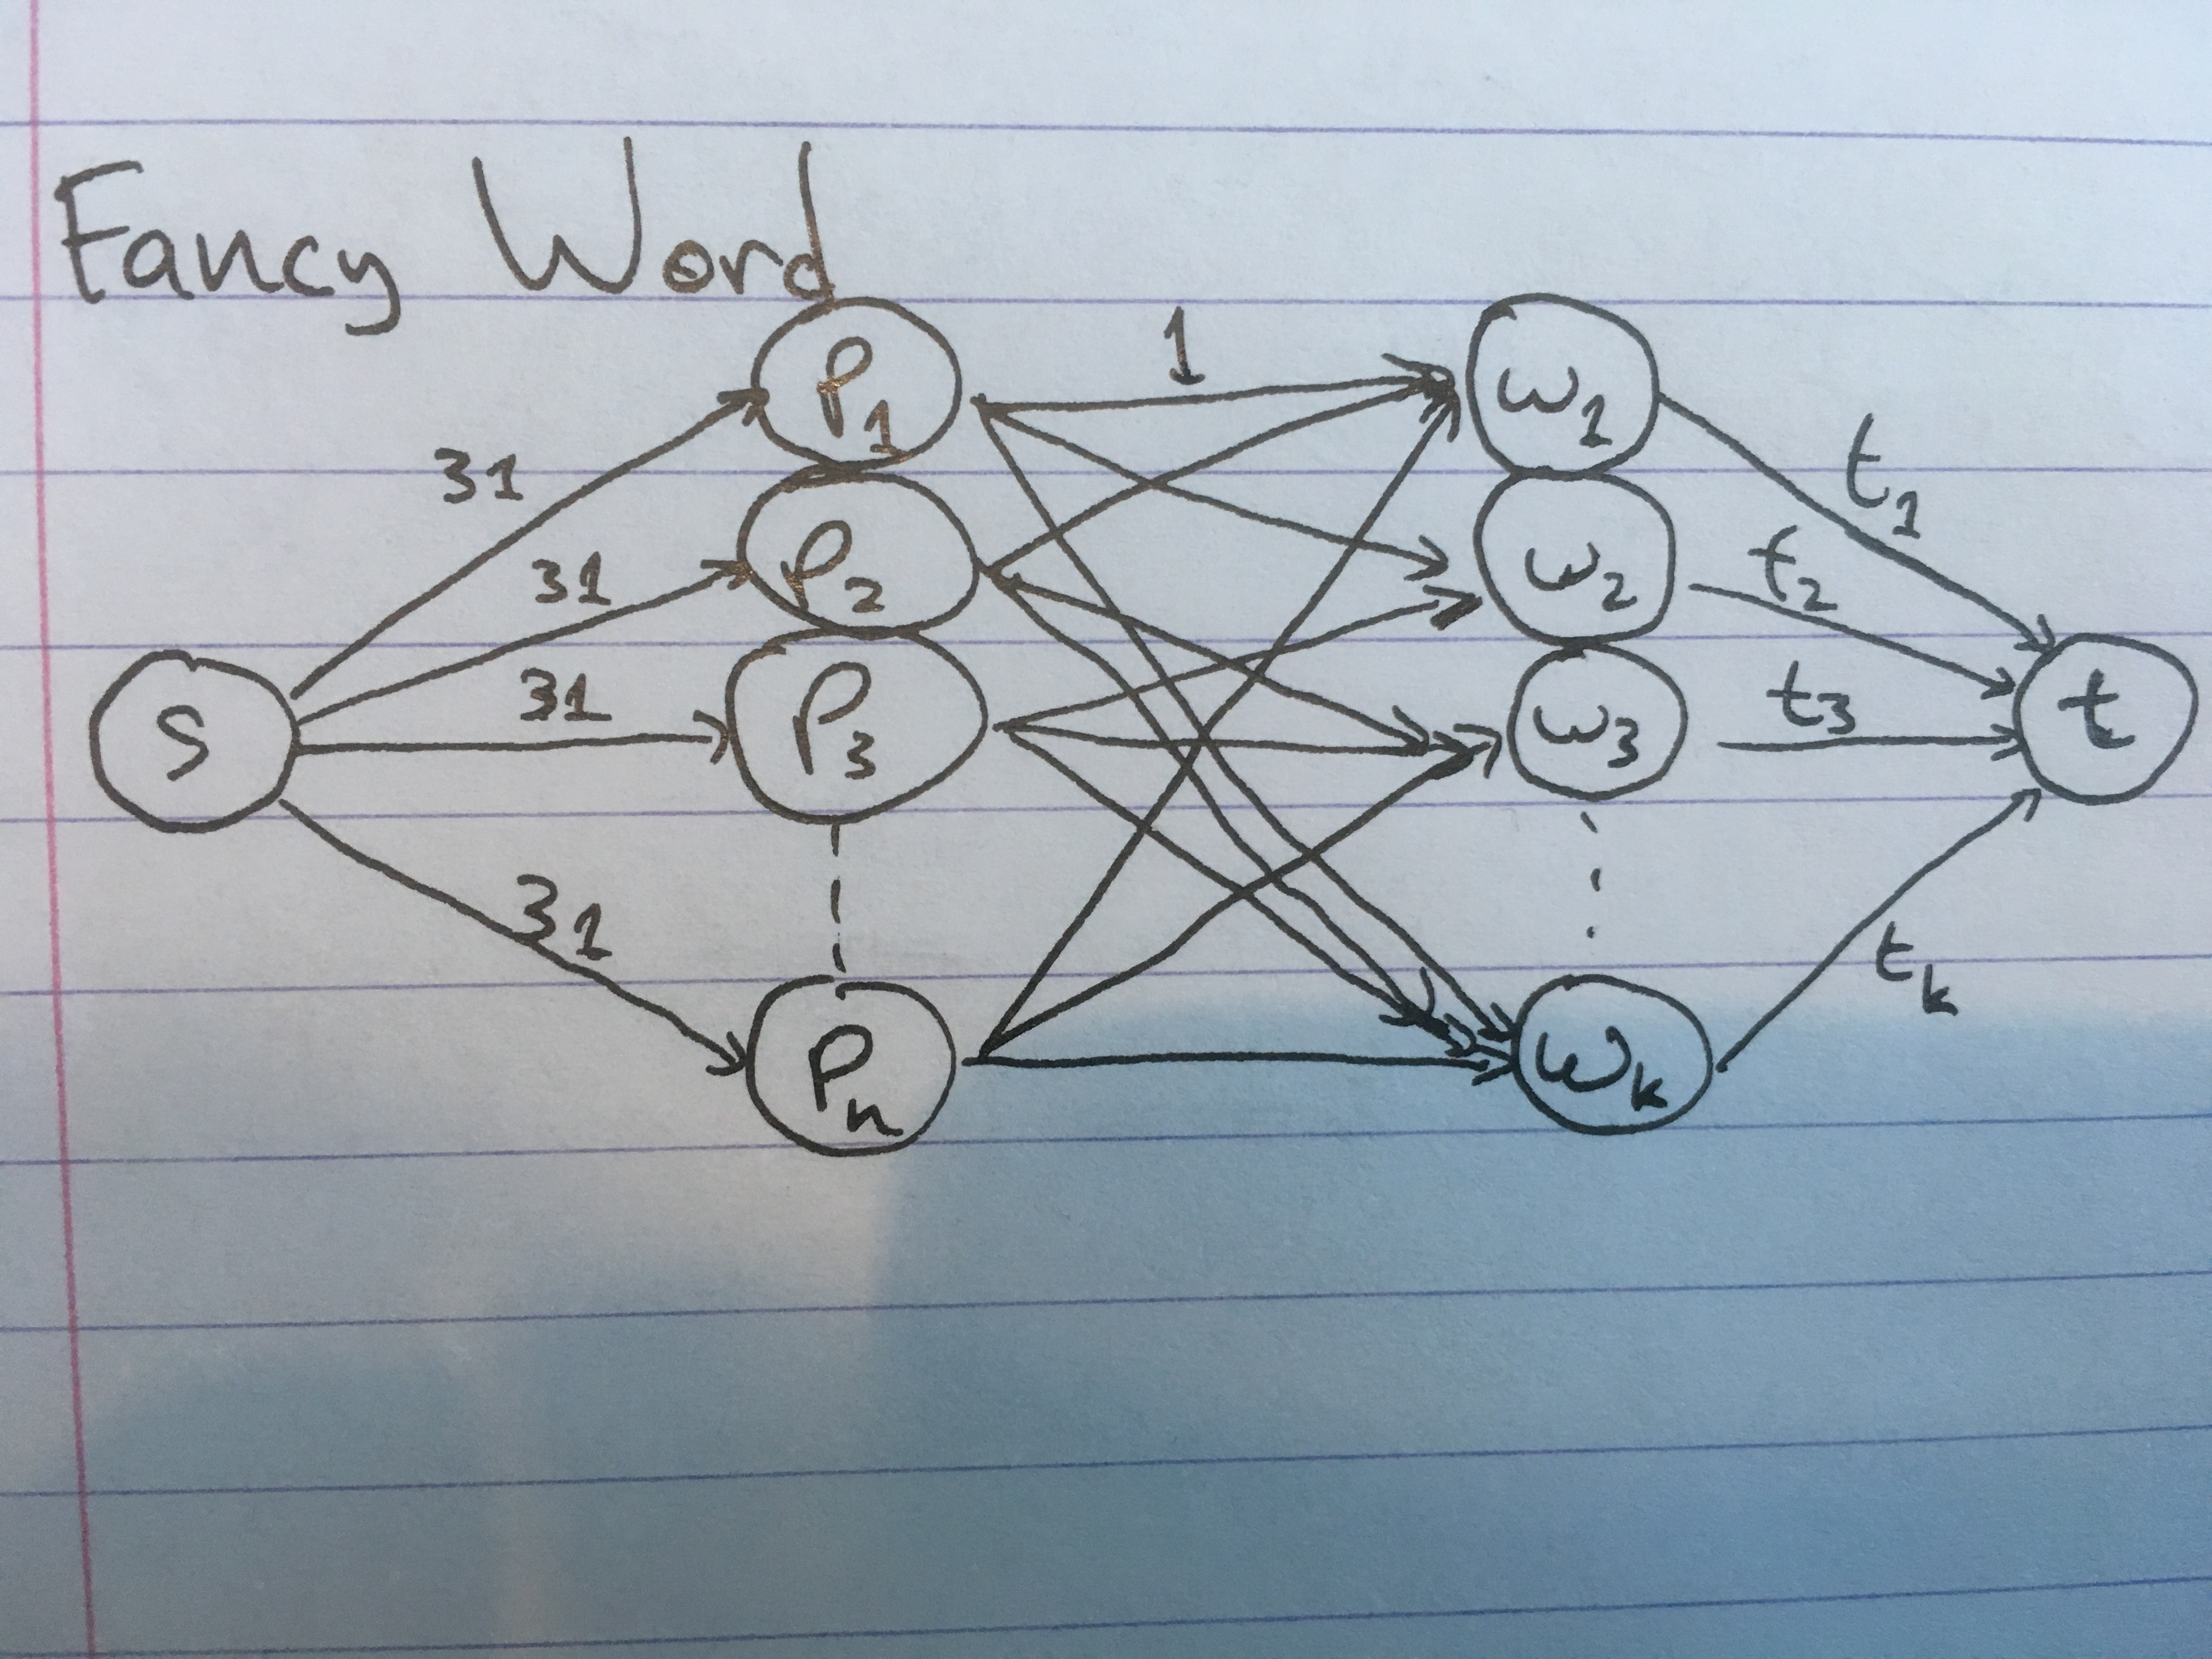
\includegraphics[width=10cm,height=10cm,keepaspectratio]{q3_fancywords}
\end{center}

\begin{claim}
If and only if we are given a max flow $f=31n$ can we construct an assignment of students to 31 words such that there are no complaints. 
\end{claim}

\begin{proof}
$f$ cannot be $> 31n$, because the flow from $s$ to each student $p_i$ has capacity 31, and there are $n$ of those edges. Since each student must be assigned $31$ words, in fact it holds that we cannot have a satisfactory assignment of students to words without a max flow $f$ bounded by $31n$. Thus, no flow $f > 31n$ could ever be sent from $s$.

Given a max flow $f = 31n$ we can determine that all edges $(s, p_i)$ are fully saturated, as the cut from $s$ to the $p_i$'s has capacity $31n$. 

Since all flow was able to traverse the edges $(p_i, w_j)$ for all $i, j$ as well as edges $(w_j, t)$ such that there is no overflow across any edges. There is no overflow since otherwise, a maxflow of $f = 31n$ would not be possible. Note that this does not necessarily mean edges $(p_i, w_j)$ or $(w_j, t)$ are saturated, merely that their capacities are at least $31n$.

Knowing these things, we can find our max flow $f$ using $Ford-Fulkerson$. Note that flow across inner edges $(p_i, w_j)$ or leaving edges $(w_j, t)$ are not integral. However, since we know that all capacities are integral and our max flow of $31n$ is a multiple of an integer and thus integral, by the Integrality Theorem, all flow can be assigned an integral value of either $(0,1)$ across the inner edges, and $(0, t_j)$  on leaving edges. Flow of $(0, 1)$ across inner edges represents an assignment of a student with some word. Flow of $(0, t_j)$ across leaving edges represent the number of times a word $w_j$ was assigned to a student. 
\end{proof}

\begin{claim}
No satisfactory (i.e. 0 complaints) pairing exists for when max flow $f < 31n$.
\end{claim}
\begin{proof}
If $31n-f$ is not an integer, then the Integrality Theorem does not hold, as flow $f$ is not integral. This means that a proper pairing is not possible as student-words pairings can not be properly defined, as assignment is determined by flow of $(0,1)$. Thus, some students will be disappointed as they cannot receive proper assignments.

If $31n-f$ is integral, then $f$ is smaller than $n$ by at least 1. This means that some flow representing a student->word assignment was not able to be established, and there will be, at the very least, 1 student with at least $1$ less word assigned to them, which is grounds for dissatisfaction.
\end{proof}

The running time is the time required to solve the max-flow problem on a graph with $O(n+k)$ nodes and $O(nk)$ edges.

\pagebreak

\section*{Solution to Problem 4 - Mi-$k$ Drop}

Let $G = (V,E)$ be a directed graph with a source $s \in V$, a sink $t \in V$, and where every edge $e \in E$ has capacity exactly 1. Let $k$ be he value of the maximum flow in $G$.

\textbf{Question:} Given an arbitrary integer $1 \leq q \leq k$, can you always remove $q$ edges from $G$ so that in the resulting graph $G'$ the value of the maximum flow is $k-q$?

\noindent\rule{17cm}{0.4pt}

Yes.

\begin{proof}
By the MaxFlow-MinCut theorem, the maximum flow in a network is bounded by $|min\text{ }cut|$, which means that if $k$ is the maximum flow in $G$, then $k$ is also $|min\text{ }cut|$. Since $|min\text{ }cut|$ acts as an upper bound on our flow, it stands that removing edges in $G$ is a perfectly valid operation as long as the number of edges removed is bounded by $1 \leq q \leq k$. Since every edge in $G$ has capacity $1$, removing any edge  reduces the maximum flow by 1. Repeat this process $q$ times, and you have a max flow reduced by $q$, aka $k-q$.
\end{proof} 

\end{document}
